\section{Simulation Results}
We now present the results of some simulations ran to verify the theoretical results and compare the models

\subsection{Data Generating Process}
\label{sec:dgp}

We generate i.i.d.\ samples $(Y_i, X_i, Z_i)_{i=1}^{n}$ from
\[
    Y_i = \beta X_i + \varepsilon_i, \qquad X_i = \mu_{ZX} Z_i + v_i,
\]
with $\beta = 2$, $\mu_{ZX} = 1$, $\sigma_v = 0.8$, and $Z_i \sim \mathrm{Uniform}\{-1,+1\}$. The errors $\varepsilon_i, v_i$ are independent of $Z_i$ and of each other.

Our baseline distribution is Pareto($\alpha = 2.1$), centred with zero mean and finite variance but no finite moments of order $2\alpha = 4.2$, placing it in the heavy-tailed regime where sub-Gaussian concentration matters most. We also consider Student-$t(3)$, Pareto($\alpha \in \{2.5, 3.5\}$), and Gaussian errors. Unless stated otherwise, the Pareto($\alpha = 2.1$) is assumed to be the baseline distribution.

Population quantities $\sigma_{Z\varepsilon} \approx 2.88$, $\sigma_{ZX} \approx 2.57$, $\mu_{ZX} \approx 1.00$ are estimated from a single sample of $n = 500{,}000$ and used for theoretical bounds throughout. Unless stated otherwise, $\delta$ is set to 0.05.


\subsection{Empirical Survival Functions}
\label{sec:sim_survival}

We draw $10{,}000$ independent samples of size $n = 2{,}000$ under Pareto($2.1$) errors and plot the empirical survival function $\hat{P}(\abs{\hat{\beta} - \beta} > t)$ for each estimator on a log--log scale (Figure~\ref{fig:survival}). For sufficiently small $\delta$, standard IV becomes the worst performing. MoR shows the steepest decay, consistent with its tighter bound found earlier.

\begin{figure}[t]
    \centering
    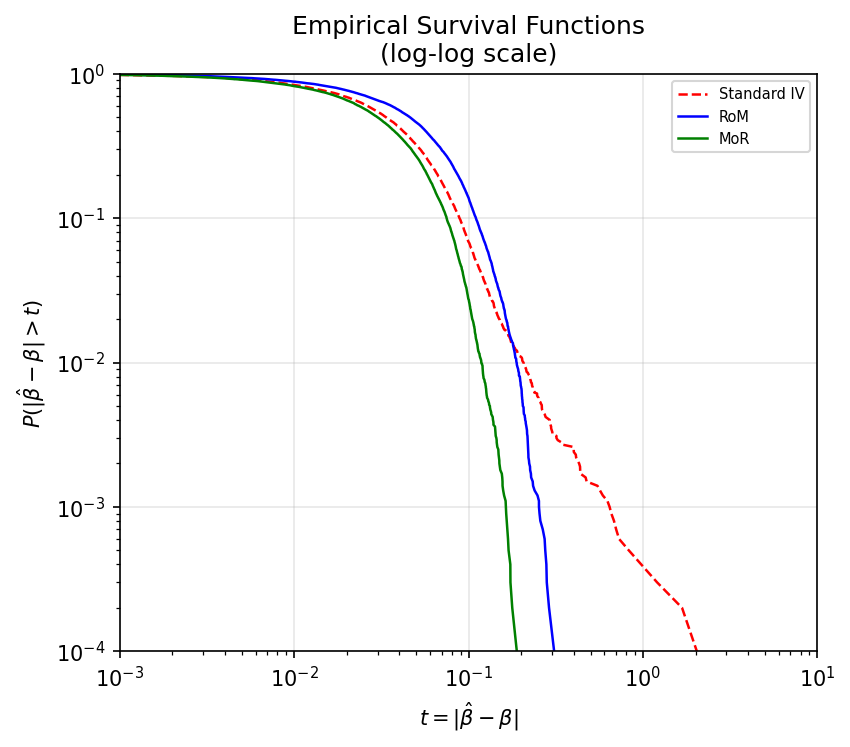
\includegraphics[width=0.7\textwidth]{images/graphs/sim_1_survival.png}
    \caption{Empirical survival functions $\hat{P}(\abs{\hat{\beta} - \beta} > t)$ on a log--log scale ($n = 2{,}000$, $k = 16$, Pareto($2.1$) errors, $10{,}000$ replications).}
    \label{fig:survival}
\end{figure}


\subsection{Bound Tightness and Coverage}
\label{sec:sim_coverage}

We assess conservativeness at failure probabilities $\delta \in \{0.01, 0.05, 0.10, 0.30, 0.50\}$. For each $\delta$ we set $k = \lceil 8\ln(1/\delta) \rceil$ (MoR) or $k = \lceil 8\ln(2/\delta) \rceil$ (RoM), compute the theoretical CI width, and measure empirical coverage over $10{,}000$ replications with $n = 2{,}000$. We report $c^*$, the smallest fraction of the theoretical width achieving coverage $\geq 1-\delta$; $1/c^*$ measures conservativeness.

Table~\ref{tab:coverage} shows all bounds achieve nominal coverage. The IV bound is $\approx 6$--$10\times$ conservative, MoR is $\approx 21$--$28\times$, and RoM is the most conservative at $\approx 50$--$70\times$.

\begin{table}[t]
\centering
\caption{Coverage validation at moderate $\delta$. $c^*$ is the smallest fraction of the theoretical half-width needed to achieve coverage $\geq 1 - \delta$; $1/c^*$ measures conservativeness.}
\label{tab:coverage}
\renewcommand{\arraystretch}{1.3}
\begin{tabular}{ccccccccc}
\toprule
 & & & \multicolumn{3}{c}{Theoretical width} & \multicolumn{3}{c}{Conservativeness ($1/c^*$)} \\
\cmidrule(lr){4-6}\cmidrule(lr){7-9}
$\delta$ & $k_{\mathrm{MoR}}$ & $m$ & IV & MoR & RoM & IV & MoR & RoM \\
\midrule
0.50 &  6 & 333 & 0.26 & 0.89 & 2.84 & $7.8\times$ & $27.8\times$ & $62.5\times$ \\
0.30 & 10 & 200 & 0.33 & 1.15 & 3.64 & $6.4\times$ & $24.4\times$ & $52.6\times$ \\
0.10 & 19 & 105 & 0.58 & 1.59 & 5.53 & $6.6\times$ & $21.7\times$ & $50.0\times$ \\
0.05 & 24 &  83 & 0.81 & 1.79 & 7.35 & $7.3\times$ & $21.3\times$ & $55.6\times$ \\
0.01 & 37 &  54 & 1.82 & 2.21 & 13.32 & $9.9\times$ & $21.3\times$ & $71.4\times$ \\
\bottomrule
\end{tabular}
\end{table}

\subsubsection{Theoretical Widths at Extreme $\delta$}
Table~\ref{tab:extreme_delta} reports theoretical CI widths for $\delta \in [10^{-1}, 10^{-8}]$ without simulation. The IV width grows as $1/\sqrt{\delta}$ while MoR grows as $\sqrt{\ln(1/\delta)}$, with a crossover near $\delta \approx 5.9 \times 10^{-3}$. At $\delta = 10^{-6}$ the IV bound is $47\times$ wider, confirming the qualitative advantage of sub-Gaussian concentration for high-confidence inference.

\begin{table}[t]
\centering
\caption{Theoretical CI widths at extreme $\delta$. MoR becomes tighter than IV for $\delta \lesssim 5.9 \times 10^{-3}$.}
\label{tab:extreme_delta}
\renewcommand{\arraystretch}{1.3}
\begin{tabular}{cccccc}
\toprule
$\delta$ & IV width & MoR width & IV/MoR ratio & $k_{\mathrm{MoR}}$ & $m$ \\
\midrule
$10^{-1}$ & 0.58 & 1.59 & 0.36 & 19 & 105 \\
$10^{-2}$ & 1.82 & 2.21 & 0.82 & 37 & 54 \\
$10^{-3}$ & 5.75 & 2.75 & 2.09 & 56 & 35 \\
$10^{-4}$ & 18.19 & 3.13 & 5.81 & 74 & 27 \\
$10^{-6}$ & 181.92 & 3.84 & 47.4 & 111 & 18 \\
$10^{-8}$ & 1819.2 & 4.51 & 403 & 148 & 13 \\
\bottomrule
\end{tabular}
\end{table}
